\documentclass[8pt,dvipsnames]{beamer}
\usepackage[T1]{fontenc}
\usepackage{libertinus}
\usepackage{amsmath}
\usepackage[most]{tcolorbox}
\usepackage{graphicx}
\usepackage{tikz}
\usetikzlibrary{positioning}

\usepackage{hyperref}
%python 
\usepackage{listings}
% Default fixed font does not support bold face
\DeclareFixedFont{\ttb}{T1}{txtt}{bx}{n}{8} % for bold
\DeclareFixedFont{\ttm}{T1}{txtt}{m}{n}{8}  % for normal

% Custom colors
\usepackage{color}
\definecolor{deepblue}{rgb}{0,0,0.5}
\definecolor{deepred}{rgb}{0.6,0,0}
\definecolor{deepgreen}{rgb}{0,0.5,0}

\usepackage{listings}

% Python style for highlighting
\newcommand\pythonstyle{\lstset{
		language=Python,
		basicstyle=\ttm,
		morekeywords={self},              % Add keywords here
		keywordstyle=\ttb\color{deepblue},
		emph={MyClass,__init__},          % Custom highlighting
		emphstyle=\ttb\color{deepred},    % Custom highlighting style
		stringstyle=\color{deepgreen},
		frame=tb,                         % Any extra options here
		showstringspaces=false
}}


% Python environment
\lstnewenvironment{python}[1][]
{
	\pythonstyle
	\lstset{#1}
}
{}

% Python for external files
\newcommand\pythonexternal[2][]{{
		\pythonstyle
		\lstinputlisting[#1]{#2}}}

% Python for inline
\newcommand\pythoninline[1]{{\pythonstyle\lstinline!#1!}}

\usepackage{xcolor}  
\newcommand{\cb}[1]{{\color{CadetBlue}#1}}

\usepackage{pgfplots}
\pgfplotsset{compat=newest}
\setlength{\parskip}{0.5em}

\usepackage{setspace}
\setstretch{1.25}  
\usetheme{Singapore}
\setbeamertemplate{navigation symbols}{}


\title{CSE574 Introduction to Machine Learning}
\subtitle{Neural Network: Forward Pass and Back-propagation}
\author{Jue Guo}
\institute{University at Buffalo}
\date{\today}

\begin{document}
\begin{frame}
    \titlepage
\end{frame}
\begin{frame}
    \frametitle{Outline}
    \tableofcontents
\end{frame}

\section{Introduction}
\begin{frame}{Introduction}
\begin{itemize}
	\item step by step forward pass (forward propagation) and backward pass (back-propagation)
	\item a single hidden layer neural network 
	\begin{itemize}
		\item solving one complete cycle of forward and back-propagation
	\end{itemize}
\end{itemize}
\end{frame}

\begin{frame}
	A simple neural network: 
	\begin{figure}
		\centering
		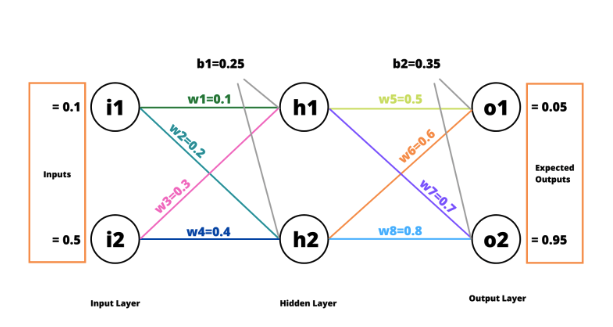
\includegraphics[width=0.8\textwidth]{imgs/nn_2.png}
	\end{figure}
\end{frame}

\subsection{Peeking inside a single neuron}
\begin{frame}{Peeking inside a single neuron}
	\begin{columns}
		\column{0.5\textwidth}
		\begin{figure}
			\centering
			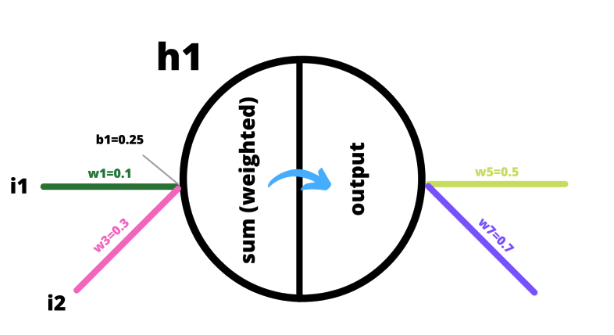
\includegraphics[width=0.8\textwidth]{imgs/nn_3.png}
		\end{figure}
		\column{0.5\textwidth}
		Inside a unit, two operations happen
		\begin{enumerate}
			\item computation of weighted sum and 
			\item squashing of the weighted sum using an activation function. 
		\end{enumerate}
		The result from the activation function (Sigmoid function (Logistic function) as the activation function.) becomes an input to the next layer (until the next layer is an Output Layer).
	\end{columns}
\end{frame}

\section{Forawrd Pass}
\begin{frame}{Forward Pass}
	For \(h_1\)
	$$
	\begin{array}{c}\operatorname{sum}_{h 1}=i_{1} * w_{1}+i_{2} * w_{3}+b_{1} \\ \operatorname{sum}_{h 1}=0.1 * 0.1+0.5 * 0.3+0.25=0.41\end{array}
	$$
	Now we pass this weighted sum through the logistic function (sigmoid
	function) so as to squash the weighted sum into the range \((0\) and +1\()\).
	The logistic function is an activation function for our example neural
	network.
	\vspace{1cm}
	
	\centering
	\textbf{What is the output?}
\end{frame}

\begin{frame}
	\begin{columns}
		\column{0.6\textwidth}
		\begin{figure}
			\centering
			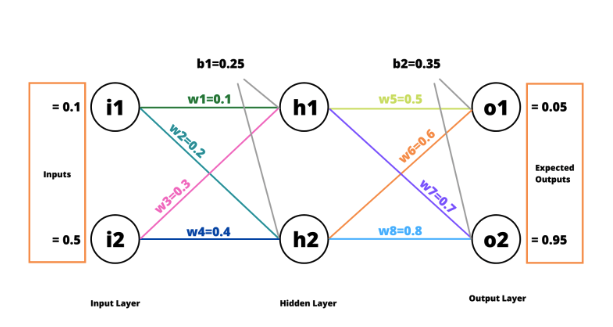
\includegraphics[width=\textwidth]{imgs/nn_2.png}
		\end{figure}
		\column{0.4\textwidth}
			$$
		\begin{array}{c}\text { output }_{h 1}=\frac{1}{1+e^{- \text {sum }_{h 1}}} \\ \text { output }_{h 1}=\frac{1}{1+e^{-0.41}}=0.60108\end{array}
		$$
		Similarly for h2, we perform the weighted sum operation \(\operatorname{sum}_{h 2}\) and compute the activation value output \({ }_{h 2}\).
		
		\centering
		\textcolor{red}{calculate...}
	\end{columns}
\end{frame}

\begin{frame}
	\begin{figure}
		\centering
		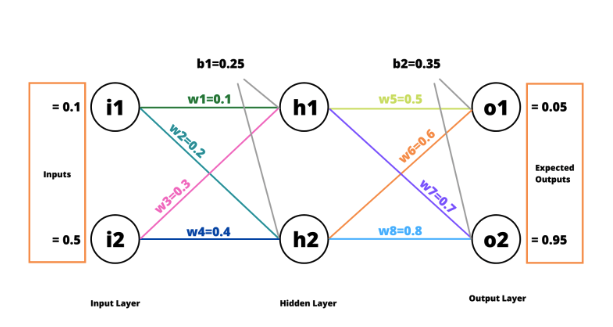
\includegraphics[width=0.6\textwidth]{imgs/nn_2.png}
	\end{figure}
	$$
	\begin{array}{c}\text { sum }_{h 2}=i_{1} * w_{2}+i_{2} * w_{4}+b_{1}=0.47 \\ \text { output }_{h 2}=\frac{1}{1+e^{- \text {sum }_{h 2}}}=0.61538\end{array}
	$$
\end{frame}

\begin{frame}
	\begin{figure}
		\centering
		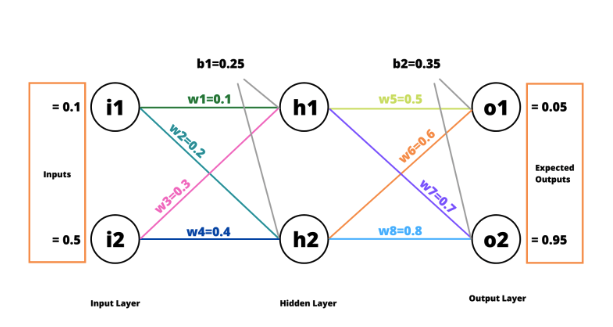
\includegraphics[width=\textwidth]{imgs/nn_2.png}
	\end{figure}
	Now do it for the output ... 
\end{frame}

\begin{frame}
	For o1, 
	$$
	\begin{array}{c}\text { sum }_{o 1}=\text { output }_{h 1} * w_{5}+\text { output }_{h 2} * w_{6}+b_{2}=1.01977 \\ \text { output }_{o 1}=\frac{1}{1+e^{- \text {sum }_{o 1}}}=0.73492\end{array}
	$$
	Similarly for o2,
	$$
	\text { sum }_{o 2}=\text { output }_{h 1} * w_{7}+\text { output }_{h 2} * w_{8}+b_{2}=1.26306
	$$
	$$
	\text { output }_{o 2}=\frac{1}{1+e^{- \text {sum }_{o 2}}}=0.77955
	$$
\end{frame}

\section{Computing the Total Error}
\begin{frame}{Computing the Total Error}
	\begin{figure}
		\centering
		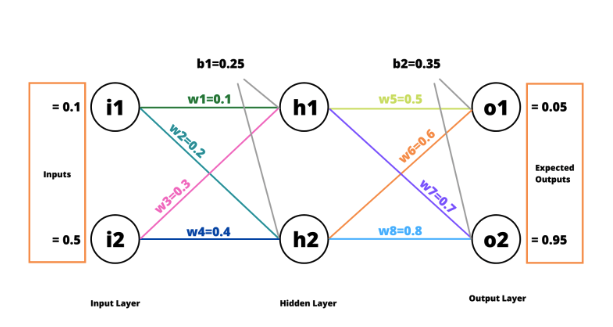
\includegraphics[width=0.6\textwidth]{imgs/nn_2.png}
	\end{figure}
	We started off supposing the expected outputs to be 0.05 and 0.95 respectively for output \({ }_{o 1}\) and output \(_{o 2}\). 
	\begin{itemize}
		\item Now we will compute the errors based on the outputs received until now and the expected outputs.
		\item Use Mean Squared Error, \textbf{Calculate} ... 
	\end{itemize}
\end{frame}

\begin{frame}
	We'll use the following error formula,
	$$
	E_{\text {total }}=\sum \frac{1}{2}(\text { target }- \text { output })^{2}
	$$
	To compute \(E_{\text {total }}\), we need to first find out respective errors at \(o 1\)
	and \(o 2\)
	$$
	E_{1}=\frac{1}{2}\left(\text { target }_{1}-\text { output }_{o 1}\right)^{2}
	$$
	$$
	E_{1}=\frac{1}{2}(0.05-0.73492)^{2}=0.23456
	$$
	Similarly for E2,
	$$
	E_{2}=\frac{1}{2}\left(\text { target }_{2}-\text { output }_{o 2}\right)^{2}
	$$
	$$
	E_{2}=\frac{1}{2}(0.95-0.77955)^{2}=0.01452
	$$
	Therefore,
	$$
	E_{\text {total }}=E_{1}+E_{2}=0.24908
	$$
\end{frame}

\section{The Back-propagation}
\begin{frame}{The Back-propagation}
	The aim of backpropagation (backward pass) is to distribute the total error back to the network so as to update the weights in order to minimize the cost function (loss). 
	\begin{itemize}
		\item The weights are updated in such as way that when the next forward pass utilizes the updated weights, the total error will be reduced by a certain margin (until the minima is reached).
	\end{itemize}
	\textbf{Chain Rule in Calculus}
	
	If we have \(y=f(u)\) and \(u=g(x)\) then we can write the derivative of \(y\) as:
	$$
	\frac{d y}{d x}=\frac{d y}{d u} * \frac{d u}{d x}
	$$
\end{frame}

\begin{frame}{w5, w6, w7, w8}
	\begin{figure}
		\centering
		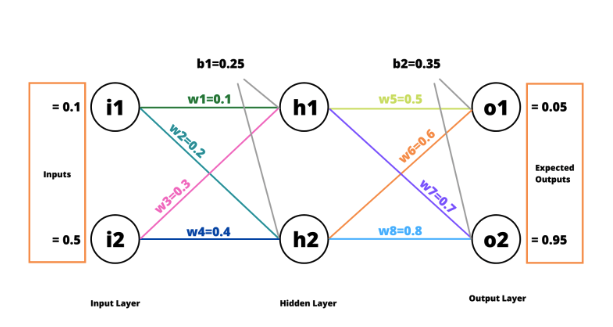
\includegraphics[width=0.5\textwidth]{imgs/nn_2.png}
	\end{figure}
	\textbf{For weights in the output layer (w5, w6, w7, w8);} Let's first see w5. If we become clear on how w5 is updated, then it would be really easy for us to generalize the same to the rest of the weights. 
	
	If we look closely at the example neural network,
	\begin{itemize}
		\item \(E_1\) is affected by \(\text{output}_{o1}\)
		\item \(\text{output}_{o1}\) is affected by \(\text {sum}_{o 1}\)
		\item \(\text {sum}_{o 1} \text { is affected by } w 5\)
	\end{itemize}
	$$
	\frac{\partial E_{\text {total }}}{\partial w 5}=\frac{\partial E_{\text {total }}}{\partial o u t p u t_{o 1}} * \frac{\partial o u t p u t_{o 1}}{\partial s u m_{o 1}} * \frac{\partial s u m_{o 1}}{\partial w 5}
	$$
\end{frame}

\subsection{Component 1: partial derivative of Error w.r.t. Output}
\begin{frame}{Component 1: partial derivative of Error w.r.t. Output}
	$$
	\begin{array}{c}E_{\text {total }}=\sum \frac{1}{2}(\text { target }- \text { output })^{2} \vspace{4pt}\\ E_{\text {total }}=\frac{1}{2}\left(\text { target }_{1}-\text { output }_{o 1}\right)^{2}+\frac{1}{2}\left(\text { target }_{2}-\text { output }_{o 2}\right)^{2}\end{array}
	$$
	Therefore, 
	\begin{equation*}
		\begin{aligned}
			\frac{\partial E_{\text {total }}}{\partial \text { output }_{o 1}}&=2 * \frac{1}{2} *\left(\text { target }_{1}-\text { output }_{o 1}\right) *-1 \\
			&=\text { output }_{o 1}-\text { target }_{1}\\
		\end{aligned}
	\end{equation*}
\end{frame}

\subsection{Component 2: partial derivative of Output w.r.t. Sum}
\begin{frame}{Component 2: partial derivative of Output w.r.t. Sum}
	The output section of a unit of a neural network uses non-linear activation functions. The activation function used in this example is Logistic Function. When we compute the derivative of the Logistic Function, we get:
	$$
	\begin{array}{c}\sigma(x)=\frac{1}{1+e^{-x}} \vspace{4pt}\\ \frac{\mathrm{d}}{\mathrm{dx}} \sigma(x)=\sigma(x)(1-\sigma(x))\end{array}
	$$
	Therefore, the derivative of the Logistic function is equal to output multiplied by (1 – output).
	$$
	\frac{\partial\text { output }_{o 1}}{\partial \text { sum }_{o 1}}=\text { output }_{o 1}\left(1-\text { output }_{o 1}\right)
	$$
\end{frame}

\subsection{Component 3: partial derivative of Sum w.r.t. Weight}
\begin{frame}{Component 3: partial derivative of Sum w.r.t. Weight}
	$$
	\text { sum }_{o 1}=\text { output }_{h 1} * w_{5}+\text { output }_{h 2} * w_{6}+b_{2}
	$$
	Therefore, 
	$$
	\frac{\partial s u m_{o 1}}{\partial w 5}=\text { output }_{h 1}
	$$
	Putting them together,
	$$
	\frac{\partial E_{\text {total }}}{\partial w 5}=\frac{\partial E_{\text {total }}}{\partial \text { output }_{o 1}} * \frac{\partial \text { output }_{o 1}}{\partial s u m_{o 1}} * \frac{\partial s u m_{o 1}}{\partial w 5}
	$$
	$$
	\frac{\partial E_{t o t a l}}{\partial w 5}=\left[\text { output }_{o 1}-\text { target }_{1}\right] *\left[\text { output }_{o 1}\left(1-\text { output }_{o 1}\right)\right] *\left[\text { output }_{h 1}\right]
	$$
	$$
	\frac{\partial E_{t o t a l}}{\partial w 5}=0.68492 * 0.19480 * 0.60108
	$$
	$$
	\frac{\partial E_{t o t a l}}{\partial w 5}=0.08020
	$$
\end{frame}

\begin{frame}
	The \(n e w \_w_{5}\) is,
	
	\(n e w_{-} w_{5}=w 5-n * \frac{\partial E_{\text {total }}}{\partial w 5}\), where \(\mathrm{n}\) is learning rate.
	
		$$
		n e w \_w_{5}=0.5-0.6 * 0.08020
		$$
		$$
		n e w \_w_{5}=0.45187
		$$
		We can proceed similarly for w6, w7 and w8. (10 minutes)
\end{frame}

\begin{frame}{w1,w2,w3,w4}
	\begin{figure}
		\centering
		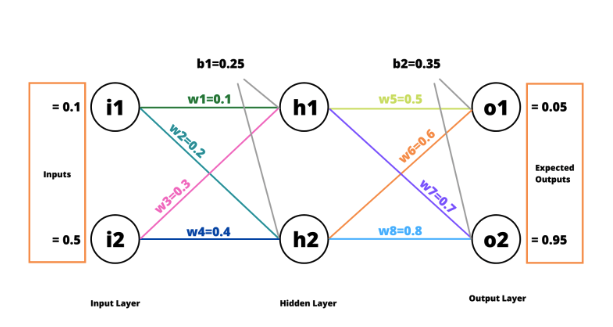
\includegraphics[width=0.6\textwidth]{imgs/nn_2.png}
	\end{figure}
	\begin{figure}
		\centering
		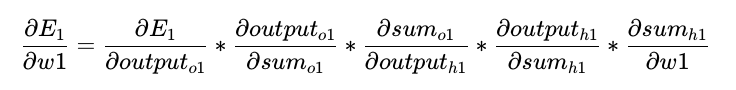
\includegraphics[width=0.6\textwidth]{imgs/nn_4.png}
		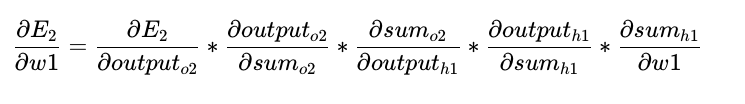
\includegraphics[width=0.6\textwidth]{imgs/nn_5.png}
	\end{figure}
\end{frame}
\end{document}